\subsection*{1. Implementando eleição de coordenador}
\addcontentsline{toc}{section}{1. Implementando eleição de coordenador}

\subsubsection{1.1 -Modificar a variável ZK de acordo com a instalação do Zookeeper em
run leader.sh. Assegurar que exista um servidor do Zookeeperfuncionando localmente.}
\addcontentsline{toc}{subsection}{1.1 Modificar a variável ZK de acordo com a instalação do Zookeeper em run leader.sh.}

\vspace{-0.5em}
\begin{minipage}{\textwidth}
  \hspace{-1em}
  \centering
  \lstinputlisting[language=sh]{pratica5/codigos/run_leader.sh}
  \label{prog1}
  \hspace{1em}
\end{minipage}
\vspace{0.5em}

\subsubsection{1.2 - Executar várias instâncias de run leader.sh. O que aconteceu?}
\addcontentsline{toc}{subsection}{1.2 Executar várias instâncias de run leader.sh.}

Conforme o processo líder mais antigo morre, o próximo líder é o processo que está olhando para o znode mais antigo que os demais restantes. \newline

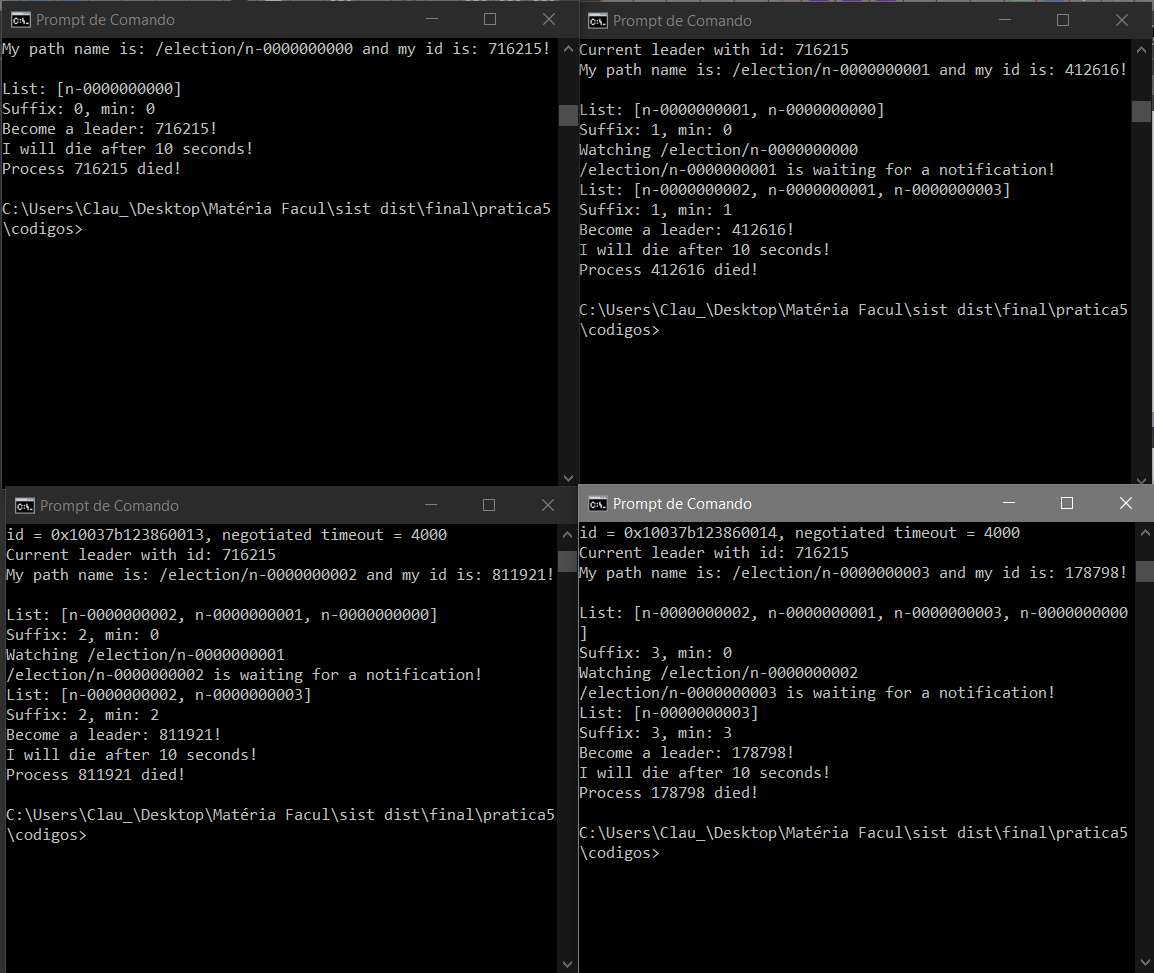
\includegraphics[width=20cm]{pratica5/prints/roteiro 1.2.PNG}

\subsubsection{1.3 - Executar várias instâncias de run leader.sh e, em seguida, matar
alguma instância intermediária. O que aconteceu?}
\addcontentsline{toc}{subsection}{2.4 Executar várias instâncias de run leader.sh. e, em seguida, matar alguma instância intermediária}

A fila é refeita após o processo intermediário ser finalizado. A cadeia de execução continua sendo executada normalmente, até o último processo que foi criado. \newline

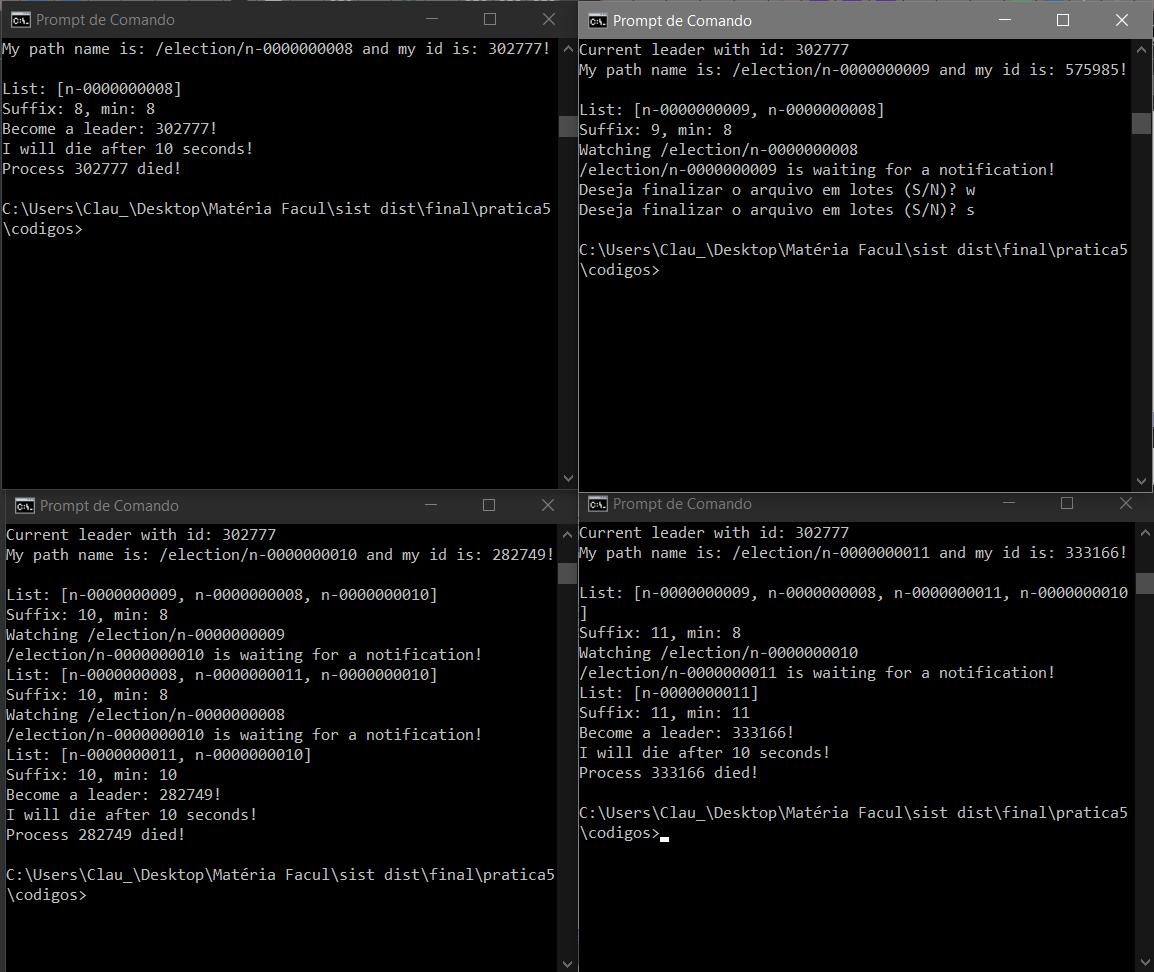
\includegraphics[width=20cm]{pratica5/prints/roteiro 1.3.PNG}


\subsection*{2. Criando um cluster para o Zookeeper – ensemble.}
\addcontentsline{toc}{section}{2. ?}

